\documentclass{beamer}
\usepackage{textcomp}
\usepackage[ngerman]{babel}
\usepackage[utf8]{inputenc}
\usepackage[T1]{fontenc}
\usepackage{fancybox}
\usepackage{graphicx}
\usepackage{hyperref}
\usepackage{amssymb}
\usepackage{amsmath}
\usepackage{amsthm}
\usepackage{listings}
\usepackage[scaled]{luximono}


\usetheme{Berlin}
\useoutertheme{infolines}
\usefonttheme{professionalfonts}
\usecolortheme{seahorse}
\usecolortheme{rose}

%\setbeamercovered{transparent}
\beamertemplatenavigationsymbolsempty
\setbeamertemplate{footline}[frame number]
\theoremstyle{example}
\newtheorem{ex}{Beispiel}
\renewenvironment{example}{\begin{ex}}{\end{ex}}


\title{Bilder In Weniger Als Tausend Worten}
\subtitle{Girlsday 2012}
\institute{Universit\"at des Saarlandes}
\date{}
\author[A. Neumann]{
	Adrian Neumann
}



\begin{document}
\lstdefinelanguage{cf}{morekeywords={shape,rule,CF,startshape,SQUARE,CIRCLE,TRIANGLE}, sensitive=true}
\lstset{basicstyle=\ttfamily\footnotesize, numbers=left, numberstyle=\tiny, language=cf}
\frame{\titlepage}

\section{Rechnen}
\begin{frame}{Rechnen}
Manipulation eines Speichers nach festen Regeln
\begin{itemize}
\item Mathe auf Papier
\item Programme in Computern
\end{itemize}
\begin{block}{}\centering
Informatiker untersuchen einfache Regelsysteme mit kompliziertem Verhalten
\end{block}
\end{frame}

\subsection{Beispiel:Game of Life}
\begin{frame}{Beispiel: Game of Life}
\begin{itemize}
\item Speicher: 
  \begin{itemize}
    \item 2D-Gitter
    \item Zellen sind ``lebendig'' (weiß) oder ``tot'' (schwarz)
  \end{itemize}
\item Regeln
  \begin{itemize}
  \item Lebendig $\rightarrow$ Tot: $<2$ oder $>3$ lebendige Nachbarn
  \item Lebendig $\rightarrow$ Lebendig: $2-3$ lebendige Nachbarn
  \item Tot $\rightarrow$ Lebendig: 3 lebendige Nachbarn
  \end{itemize}
\end{itemize}
\begin{block}{}\centering
\centering In Game of Life kann ein beliebiger Computer simuliert werden.
\end{block}
\end{frame}

\begin{frame}{Beispiel: Game of Life}
\onslide*<1>{\begin{center}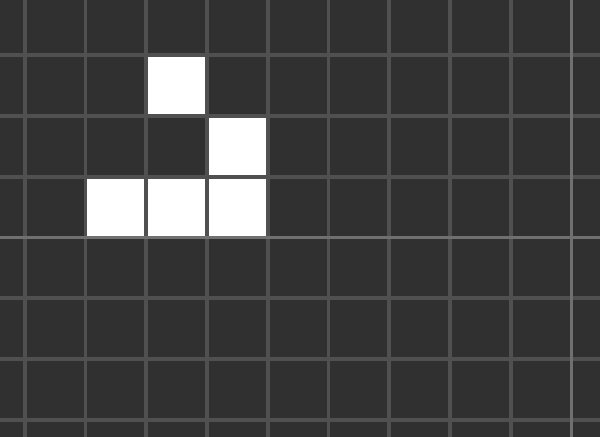
\includegraphics[width=0.8\linewidth]{./images/glider1.png}\end{center}}
\onslide*<2>{\begin{center}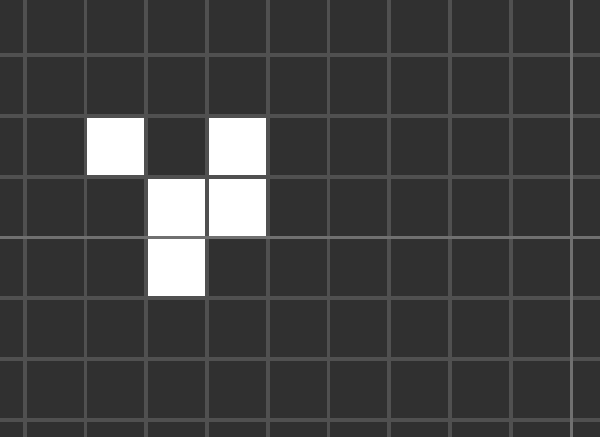
\includegraphics[width=0.8\linewidth]{./images/glider2.png}\end{center}}
\onslide*<3>{\begin{center}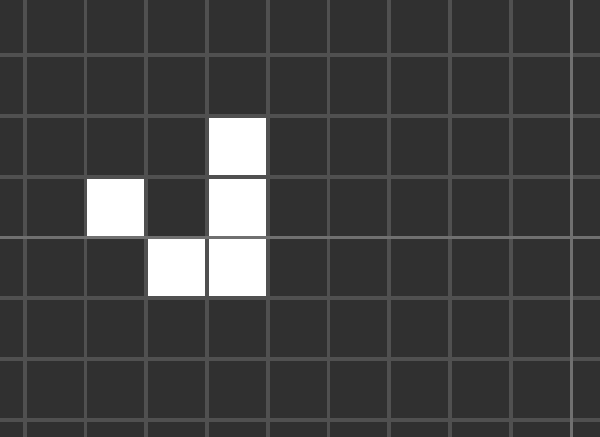
\includegraphics[width=0.8\linewidth]{./images/glider3.png}\end{center}}
\onslide*<4>{\begin{center}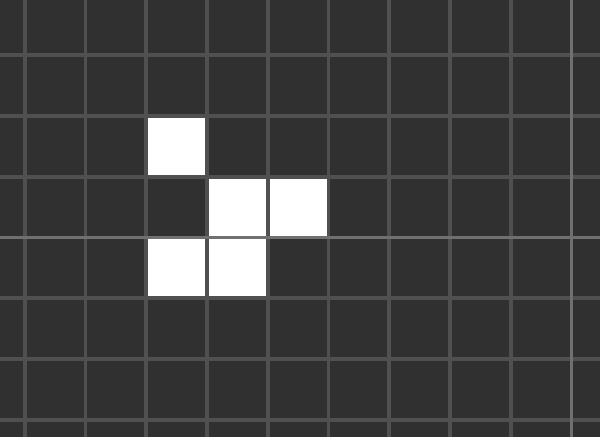
\includegraphics[width=0.8\linewidth]{./images/glider4.png}\end{center}}
\onslide*<5>{\begin{center}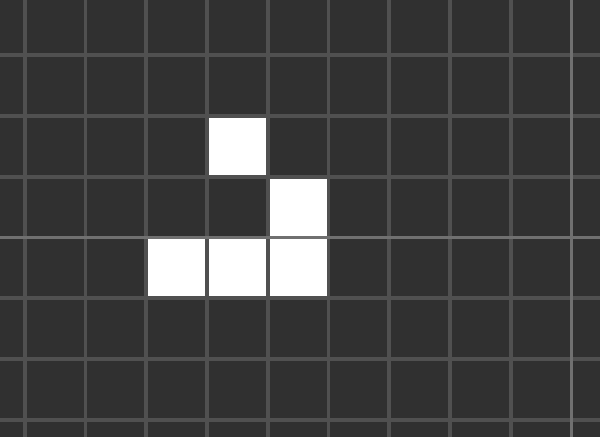
\includegraphics[width=0.8\linewidth]{./images/glider5.png}\end{center}}
\onslide*<6>{\begin{center}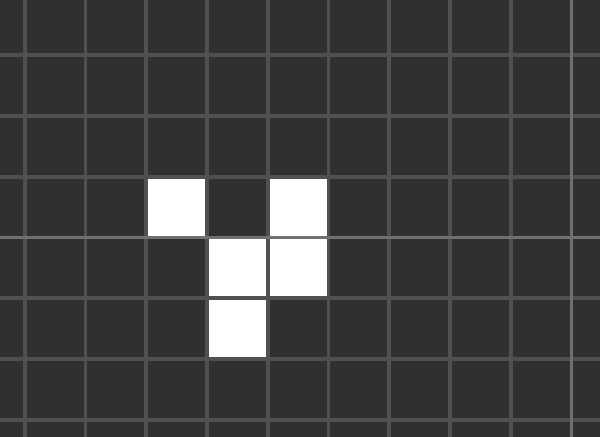
\includegraphics[width=0.8\linewidth]{./images/glider6.png}\end{center}}
\onslide*<7>{\begin{center}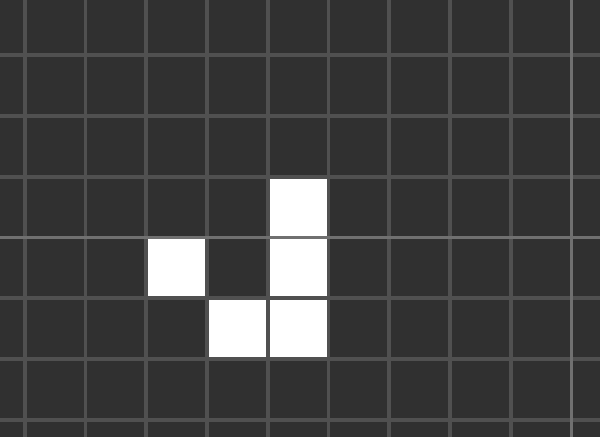
\includegraphics[width=0.8\linewidth]{./images/glider7.png}\end{center}}
\onslide*<8>{\begin{center}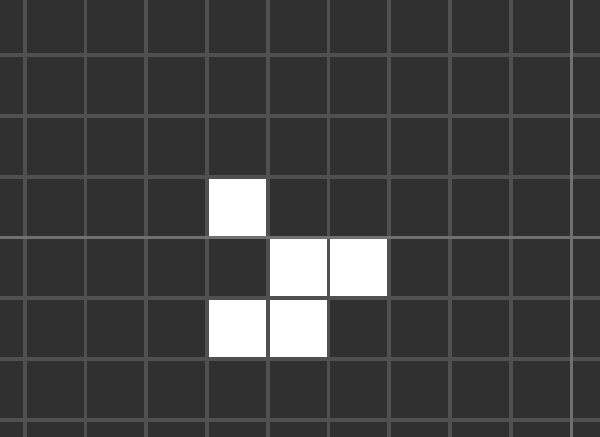
\includegraphics[width=0.8\linewidth]{./images/glider8.png}\end{center}}
\onslide*<9>{\begin{center}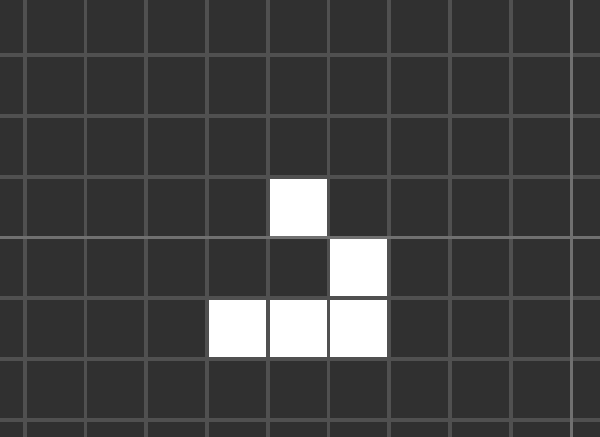
\includegraphics[width=0.8\linewidth]{./images/glider9.png}\end{center}}

\end{frame}

\section{Arbeiten mit ``Sprachen''}
\begin{frame}
  \begin{definition}
    \begin{description}
    \item[Alphabet:] Endliche Menge von ``Buchstaben''
    \item[Wort:] Endliche Sequenz von Buchstaben
    \item[Sprache:] Menge von Wörtern (i.\,d.\,R.\ unendlich)
    \end{description}
  \end{definition}
  \begin{example}
    \begin{description}
    \item[Alphabet:] $\Sigma = \{ (,)\}$
    \item[Wort:] $()(())$ oder $((())$ oder $))(($ \ldots
    \item[Sprache:] $L=\{w | \text{$w$ ist korrekt geklammert}\}$
      $L = \{(),(()),()(),(())(),\ldots\}$
    \end{description}
  \end{example}
\end{frame}

\subsection{Grammatiken}
\begin{frame}{Grammatiken}
  \begin{itemize}
  \item Einfache Regeln zum Beschreiben von Sprachen
  \item ``Grammatik'' wie in der Schule: Irreführend
  \item Zwei Arten von Symbolen:
    \begin{itemize}
    \item Buchstaben (\emph{Terminalzeichen}): hier Kleinbuchstaben $a,b,c$
    \item Platzhalter (\emph{Nichtterminalzeichen}): hier Großbuchstaben $A,B,C$

      Ein Nichtterminalzeichen ist besonders: Das \emph{Startsymbol}
    \end{itemize}
  \item Regeln um Wörter zu erzeugen
  \item Sprache: Menge aller Wörter, die man mit der Grammatik erzeugen kann
  \end{itemize}
\end{frame}

\subsection{Produktionsregeln}
\begin{frame}{Produktionsregeln}
  \begin{itemize}
  \item Regeln haben die Form
    \[\text{\textit{String}}_1 \longrightarrow \text{\textit{String}}_2\]
  \item Darf linke Seite durch rechte Seite ersetzen
  \item Angefangen wird mit dem Startsymbol
  \item Prozess ist abgeschlosesn, wenn kein Nichtterminal übrig ist
  \end{itemize}
\hspace{2cm} Heute: \emph{Kontextfreie} Grammatiken

\hspace{2cm} \textit{String$_1$} ist genau ein Nichtterminal

\end{frame}

\subsection{Beispiel: Klammerausdrücke}
\begin{frame}{Beispiel}
  \begin{itemize}
  \item Schon gesehen: $\Sigma = \{(,)\}$ und  $L = \{ w | \text{$w$ ist korrekt geklammert}\}$
  \item Grammatik:
    \begin{columns}[l]
     \column{2cm}
    \begin{align*}
      S &\rightarrow ()\\
      S &\rightarrow SS\\
      S &\rightarrow (S)
    \end{align*}
     \column{6cm}
     \begin{ex}
       \vspace*{5cm}
       \hspace*{6cm}
     \end{ex}
    \end{columns}
  \end{itemize}
\end{frame}

\subsection{Mehr als Buchstaben}
\begin{frame}{Mehr als Buchstaben}
  \begin{itemize}
  \item Besonderes Alphabet
    \begin{itemize}
    \item Geometrische Primitive (Rechteck, Dreieck, Ellipse)
    \item Rotationen
    \item Skalierungen
    \item Translationen
    \item Farbveränderungen
    \end{itemize}
  \item Grammatik regelt, wie daraus Bilder erzeugt werden
  \end{itemize}
\end{frame}

\subsection{Context-Free Art}
\begin{frame}[fragile]{Beispiel}
\begin{columns}
\column{4cm}
\footnotesize{
\begin{lstlisting}
CF::Background = [b -1]
startshape T[
  b 1 a -1 sat 1 h 310
]

shape T
rule {
  SQUARE[x .5 y -.05 s 1 .1]
  CIRCLE[x 1.77 y .13 s .5]
  T[r -2.07028 s 0.298966
    a .1 h 90 sat -.3]
  T[x 1 r 45.9297 s .324258
    a .1 sat .1]
  T[x 1.72574 y .806014
    r -48 s .922]
} 
\end{lstlisting}
}
\column{6cm}
\hfill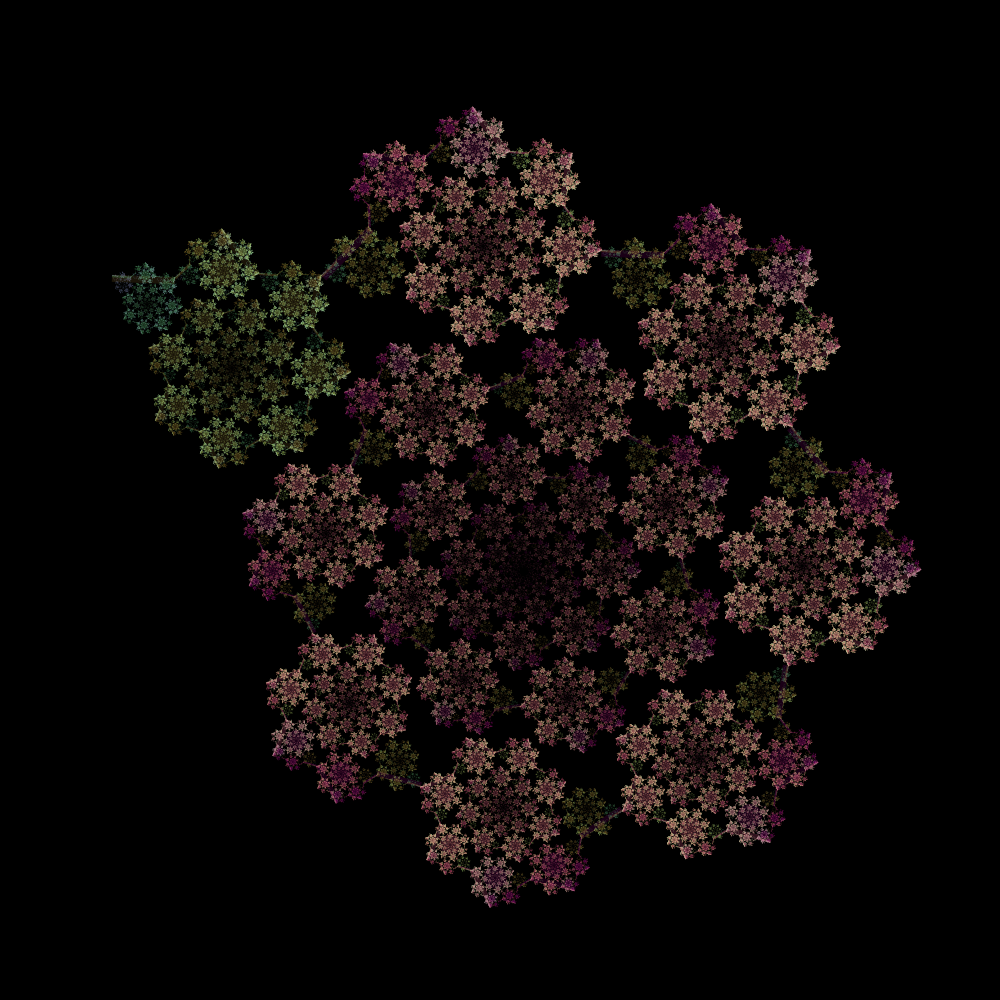
\includegraphics[width=\linewidth]{./images/beispiel.png}
\end{columns}
\tiny
\hfill CC-BY-SA 3.0 zol
\end{frame}

\begin{frame}{Steueranweisungen}
Einstellungen für das ganze Bild:
  \begin{itemize}
  \item Beginnen mit \lstinline!CF::!
    \begin{itemize}
    \item Hintergrund: \lstinline!CF::Background!
    \item Minimalgröße der Bildelemente: \lstinline!CF::MinimumSize!
    \item[\vdots]
    \end{itemize}
   \item Im Beispiel: \lstinline!CF::Background = [b -1]!

     Setze \textbf{b}rightness (Helligkeit) auf Minimalwert (=Schwarz).
  \end{itemize}
Startsymbol: 
\begin{itemize}
\item Festgelegt mit \lstinline!startshape!
\end{itemize}
\end{frame}

\begin{frame}{Nichtterminale}
  \begin{itemize}
  \item Heißen jetzt \lstinline!shape!
  \item Produktionsregeln werden mit \lstinline!rule! definiert.
  \item Im Beispiel
    \begin{itemize}
    \item Ein Nichtterminal: \lstinline!T!
    \item Eine Produktionsregel: Ein \lstinline!T! wird ersetzt durch
      \begin{itemize}
      \item Ein Viereck \lstinline!SQUARE!
      \item Einen Kreis \lstinline!CIRCLE!
      \item Drei \lstinline!T!
      \end{itemize}
    \end{itemize}
  \item Mehrere \lstinline{rule} können hintereinander stehen.
  \item Welche Regel angewendet wird, wird \emph{zufällig} entschieden
  \item Fertig: Keine Nichtterminale mehr \emph{oder} Alle Bildelemente zu klein
  \end{itemize}
\end{frame}

\begin{frame}{Terminale}
\begin{columns}
\column{4cm}
  Drei verschiedene Terminale:
  \begin{enumerate}
  \item \lstinline!CIRCLE!
  \item \lstinline!SQUARE!
  \item \lstinline!TRIANGLE!
  \end{enumerate}
 Alle haben Seitenlänge 1
\column{6cm}
\begin{center}
\fbox{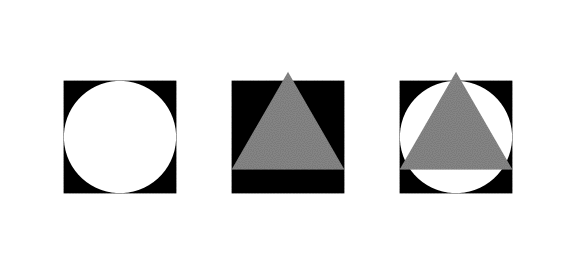
\includegraphics[width=\linewidth]{./images/Shape_demo.png}}\\\bigskip
Code für dieses Bild: Übung!
\end{center}

\end{columns}
\end{frame}

\begin{frame}{Transformationen}
  \begin{itemize}
  \item Für Matheprofis: Affine Transformation + Farbveränderung
  \item Hinter jedem Element, eckige Klammern mit Anweisungen
  \item Notationsreihenfolge egal. Immer: 1. Verschieben, 2. Rotieren, 3. Skalieren, 4. Reflektieren
  \item Doppelte Klammern: Reihenfolge zählt
  \end{itemize}
\end{frame}

\begin{frame}{Transformationen}
\begin{block}{Übersicht: Form}
  \begin{description}
  \item[Verschieben] \lstinline!x!, \lstinline!y! mit einer Zahl dahinter
  \item[Rotieren] \lstinline!r! mit Winkel (Grad) dahinter
  \item[Skalieren] \lstinline!s! mit Skalierungsfaktor dahinter. Zwei Zahlen: x,y-Richtung getrennt skalieren
  \item[Reflektieren] \lstinline!f! (flip) mit Winkel dahinter: Reflektion an Ursprungsgeraden
  \end{description}
\end{block}
\begin{block}{Übersicht: Farbe}
  \begin{description}
  \item[Farbton]
  \item[Sättigung]
  \item[Helligkeit]
  \item[Transparenz] 
  \end{description}
\end{block}
\end{frame}

\end{document}